In tabelul de mai jos, se prezinta o analiza comparativa intre fisierul obtinut in
urma rularii noastre si cel obtinut in cadrul competitiei. Am atasat si fisierele
care le puteti observa pe linkurile urmatoare: 
\href{https://docs.google.com/spreadsheets/d/1iGJHwePCzW0axJIwVes_eiN3R4ppvNu-ndrO_Fy5dL0/edit#gid=1265769327}{Link rezultate competitie }
\href{https://docs.google.com/spreadsheets/d/1kSxunni8qgQLT6ZkCRWvSO2VMy2Hz7qA/edit#gid=1476783028}{Link rezultate echipa}

\begin{figure}[h]
\centering 
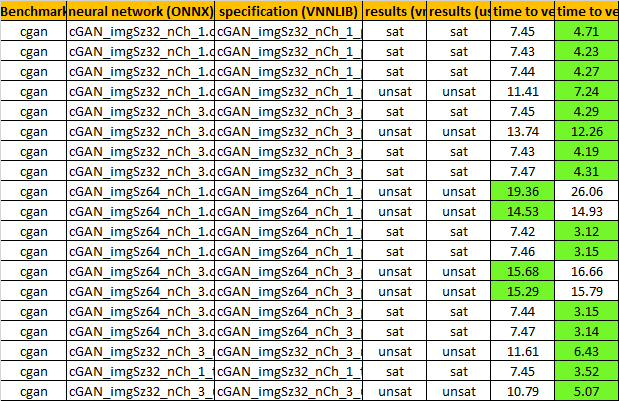
\includegraphics[width=0.8\linewidth]{imagini/interpretare rezultate/abC_comp_vs_us.png}
\caption{Rezultate alpha-beta-CROWN}
\label{fig:image1} 
\end{figure}

Putem observa faptul ca pentru fiecare intrare, rezultatele(sat/unsat) au fost aceleasi. Diferenta dintre competitie si echipa este reprezentata de timpul de verificare. Timpul de verificare înregistrat al echipei este mai mic cu aproximativ 3
secunde pentru intrările unde rezultatul este satisfiabil. În schimb, pentru intrările cu rezultat nesatisfiabil timpul de verificare este considerabil mai mare.


